%; whizzy chapter
% -initex iniptex -latex platex -format platex -bibtex jbibtex -fmt fmt
% 以上 whizzytex を使用する場合の設定。

%     Kansai Debian Meeting resources
%     Copyright (C) 2007 Takaya Yamashita
%     Thank you for Tokyo Debian Meeting resources

%     This program is free software; you can redistribute it and/or modify
%     it under the terms of the GNU General Public License as published by
%     the Free Software Foundation; either version 2 of the License, or
%     (at your option) any later version.

%     This program is distributed in the hope that it will be useful,
%     but WITHOUT ANY WARRANTY; without even the implied warranty of
%     MERCHANTABILITY or FITNESS FOR A PARTICULAR PURPOSE.  See the
%     GNU General Public License for more details.

%     You should have received a copy of the GNU General Public License
%     along with this program; if not, write to the Free Software
%     Foundation, Inc., 51 Franklin St, Fifth Floor, Boston, MA  02110-1301 USA

%  preview (shell-command (concat "evince " (replace-regexp-in-string "tex$" "pdf"(buffer-file-name)) "&"))
% 画像ファイルを処理するためにはebbを利用してboundingboxを作成。
%(shell-command "cd image200708; ebb *.png")

%%ここからヘッダ開始。

\documentclass[mingoth,a4paper]{jsarticle}
\usepackage{kansaimonthlyreport}
\usepackage[dvips]{xy}
\usepackage{ulem}

% 日付を定義する、毎月変わります。
\newcommand{\debmtgyear}{2014}
\newcommand{\debmtgdate}{25}
\newcommand{\debmtgmonth}{5}
\newcommand{\debmtgnumber}{84}

\def\fixme#1{{\color{red}{#1}}}

\begin{document}

\begin{titlepage}

% 毎月変更する部分、本文の末尾も修正することをわすれずに

 第\debmtgnumber{}回 関西 Debian 勉強会資料

\vspace{2cm}

\begin{center}
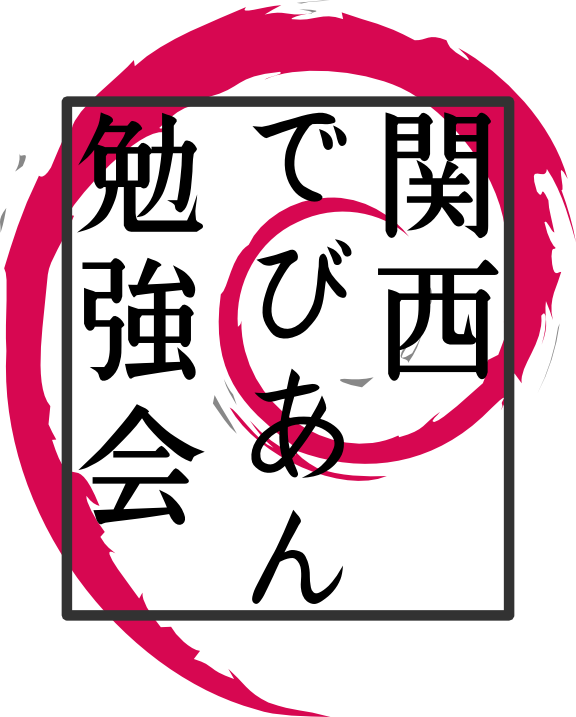
\includegraphics{image200802/kansaidebianlogo.png}
\end{center}

\begin{flushright}
\hfill{}関西 Debian 勉強会担当者 佐々木・倉敷・のがた・かわだ・八津尾 \\
\hfill{}\debmtgyear{}年\debmtgmonth{}月\debmtgdate{}日
\end{flushright}

\thispagestyle{empty}
\end{titlepage}

\dancersection{Introduction}{Debian JP}

\vspace{1em}

 関西Debian勉強会はDebian GNU/Linuxのさまざまなトピック
 (新しいパッケージ、Debian特有の機能の仕組、Debian界隈で起こった出来事、
 などなど)について話し合う会です。

 目的として次の三つを考えています。
 \begin{itemize}
  \item MLや掲示板ではなく、直接顔を合わせる事での情報交換の促進
  \item 定期的に集まれる場所
  \item 資料の作成
 \end{itemize}

 それでは、楽しい一時をお過ごしください。

\newpage

\begin{minipage}[b]{0.2\hsize}
 {\rotatebox{90}{\fontsize{80}{80}
{\gt 関西 Debian 勉強会}}}
\end{minipage}
\begin{minipage}[b]{0.8\hsize}
\hrule
\vspace{2mm}
\hrule
\setcounter{tocdepth}{1}
\tableofcontents
\vspace{2mm}
\hrule
\end{minipage}

\dancersection{最近のDebian関係のイベント報告}{Debian JP}

\subsection{第83回関西Debian勉強会}

83回目の関西Debian勉強会は4月27日(日)に、福島区民センターで行なわれまし
た。

川江さんによる「自宅サーバにKVMを導入してみよう」とDavid Bremnerさんに
よる「Notmuch Mail」の二本立てでした。

ここしばらく行なっていなかったセッション形式、また海外からのDebian
Developerの来訪となった勉強会でした。

非常に楽しそうな内容でしたが参加できなかったのが残念です。

\subsection{第113回東京エリアDebian勉強会}

113回目の東京エリアDebian勉強会は5月17日(土)に株式会社スクウェア・エニッ
クス 会議室で行なわれました。

野島さんによる「debian と docker.io」ともくもくの会の形式で行なわれまし
た。

Debianでdockerを使ってみて、Google Compute Engineでも動かしてみようとい
う内容になっています。流行りのimmutable infrastructureをDebianでdocker.io
を使って試してみてください。

\subsection{Debian Project}

\subsubsection{Code of Conduct}

ここ数ヶ月触れてきたように、Debian Projectは、GR(General Resolution:一般決議)
をへてCode of Conductが採択されました。
投票結果は「一般決議: 利用上の注意」
\footnote{\url{https://www.debian.org/vote/2014/vote_002}}
に詳しいですが、Code of Conductに大多数が賛成だったものの、その改訂を
DPL(Debian Project Leader)が行なうか、GRを通して行なうかは僅か13票差
でGRを通して行なうことになりました。

systemd関連のフレームがメーリングリスト上で起こったことに端を発して
Code of Conductをとの流れになりましたが、採択直後にまた200件を越える
systemd関連のスレッドがdebian-develにたっていたりします。

\subsubsection{systemd/GNOME Sprint}

4月25日から27日にかけて、ベルギーのアントワープで「systemd/GNOME Sprint」
\footnote{\url{https://wiki.debian.org/Sprints/2014/SystemdGNOMESprint}}
が開催されました。

「Bits from the systemd + GNOME sprint」
\footnote{\url{https://lists.debian.org/debian-devel-announce/2014/05/msg00001.html}}
の報告によると、systemd関連ではudevの整理、git-buildpackageの利用とリポ
ジトリの整理、バージョン208のパケージング、GNOME関連では、各パッケージ
の移行、VCSのSubversionからgitへの移行の検討、jessieでのGNOME 3.14の可
能性、Bluez5への取り組み、などなどが行なわれました。

systemdとGNOMEといえば筆者は最近、
\debianbug{747210}「gdm3: fails to restart X server after first logout, screen blank」
に遭遇したのでinitをsystemdに変更して回避したら、
\debianbug{746358}「systemd: system boot hangs if /etc/fstab contains an NFS mount」
に遭遇するというコンボにハメられました。

\subsubsection{リリースに向けて}
「Bits from the Release Team - Freeze, removals and archs」
\footnote{\url{https://lists.debian.org/debian-devel-announce/2014/05/msg00000.html}}
でリリースチームから6ヶ月を切ったjessieのフリーズまでのタイムテーブル
が報告されました。また各アーキテクチャの状態もあわせて報告されています。

中でもHurdについては「Bits from the Debian GNU/Hurd porters」
\footnote{\url{https://lists.debian.org/debian-devel-announce/2014/05/msg00006.html}}
で、Debian GNU/HurdでDebianの約8割のパッケージを使用できること(Iceweasel
も29でSSLが使えます)、initシステムをSysVinitに変更したこと、pthreadになっ
たこと、ネットワークドライバがDDE(Device Driver Environment)フレームワー
クベースになったこと、などなどが報告されています。

報告には挙がっていないアーキテクチャですが、arm64とmips64elも活発に開発
が進んでいるようです。
arm64については
「Arm64 port live on debian-ports」
\footnote{\url{https://lists.debian.org/debian-devel/2014/04/msg00509.html}}
と「arm64 update - help wanted」
\footnote{\url{https://lists.debian.org/debian-devel/2014/05/msg00666.html}}
によると、2つのbuilddを走らせており、4200のソースパッケージがビルドでき
ています。
mips64elについては
「mips64el: FTBFS list and buildlogs」\footnote{\url{https://lists.debian.org/debian-devel/2014/04/msg00809.html}}
によると、7000以上のパッケージのビルドに成功しており、1000以上がビルド
待ちとなっています。

\subsubsection{CTTE}
「Maximum term for tech ctte members」
\footnote{\url{https://lists.debian.org/debian-project/2014/05/msg00054.html}}
でCTTEのメンバーに任期を設けてはどうかという議題があがっています。

CTTEとはDebian Technical Committee\footnote{\url{https://www.debian.org/devel/tech-ctte}}
というDebianプロジェクト内の技術的な論争に最終的な決断を下す集団です。
最近ではJessieのLinuxアーキテクチャでのデフォルトinitシステムをsystemd
にするべきとの決定をしています。

任期を何年にするか、現行制度からどのように移行するか、まだ議論ははじまっ
たばかりですが、概ね賛同する意見が多いようです。
ちなみに、現メンバーでの最古参はIan Jacksonさんで15年5ヶ月目になります。

\subsubsection{debian-devel}
\begin{itemize}
\item 「Call for help from KDE Team」\footnote{\url{https://lists.debian.org/debian-devel/2014/05/msg00008.html}}\\
  KDEチームからのヘルプ要請。

\item 「Ghostscript licensing changed to AGPL」\footnote{\url{https://lists.debian.org/debian-devel/2014/05/msg00144.html}}\\
  GhostscriptのライセンスがAGPLに変っていたので関連パッケージに影響があ
  るのではないか。

\item 「Removal of emacs23 from unstable/testing」\footnote{\url{https://lists.debian.org/debian-devel/2014/05/msg00167.html}}\\
  Jessieフリーズ前にemacs23を除去したい。

\item 「systemd-fsck?」\footnote{\url{https://lists.debian.org/debian-devel/2014/05/msg00255.html}}\\
  systemdは全てを乗っ取る気か?から始まった200件を越えるスレッド。読んでない。

\item 「Media type vnd.debian.binary-package accepted by the IANA.」\footnote{\url{https://lists.debian.org/debian-devel/2014/05/msg00792.html}}\\
  メディアタイプにDebianのバイナリパッケージである.debと.udebが登録された。

\item 「Bug\#747596: ITP: liblxqt-mount -- Library used to manage removable devices for LXDE-Qt」\footnote{\url{https://lists.debian.org/debian-devel/2014/05/msg00314.html}}\\
  「Bug\#747597: ITP: lxqt-config -- LXQt system settings center」\footnote{\url{https://lists.debian.org/debian-devel/2014/05/msg00315.html}}\\
  「Bug\#747598: ITP: lxqt-config-randr -- Qt config GUI for X11 RandR for LXQt system settings」\footnote{\url{https://lists.debian.org/debian-devel/2014/05/msg00316.html}}\\
  「Bug\#747599: ITP: lxqt-common -- Common files for LXQt」\footnote{\url{https://lists.debian.org/debian-devel/2014/05/msg00317.html}}\\
  「Bug\#747600: ITP: lxqt-about -- The standalone LXQt "About" dialog」\footnote{\url{https://lists.debian.org/debian-devel/2014/05/msg00318.html}}\\
  「Bug\#747601: ITP: lxqt-globalkeys -- Daemon used to register global keyboard shortcuts」\footnote{\url{https://lists.debian.org/debian-devel/2014/05/msg00319.html}}\\
  「Bug\#747602: ITP: lxqt-notificationd -- The LXQt notification daemon」\footnote{\url{https://lists.debian.org/debian-devel/2014/05/msg00320.html}}\\
  「Bug\#747603: ITP: lxqt-openssh-askpass -- OpenSSH user/password GUI dialog for LXQt」\footnote{\url{https://lists.debian.org/debian-devel/2014/05/msg00321.html}}\\
  「Bug\#747604: ITP: lxqt-qtplugin -- LXDE-Qt platform integration plugin for Qt」\footnote{\url{https://lists.debian.org/debian-devel/2014/05/msg00322.html}}\\
  「Bug\#747605: ITP: pcmanfm-qt -- File manager and desktop icon manager (Qt port of PCManFM and libfm)」\footnote{\url{https://lists.debian.org/debian-devel/2014/05/msg00323.html}}\\
  「Bug\#747607: ITP: lxqt-policykit -- The LXQt PolicyKit agent」\footnote{\url{https://lists.debian.org/debian-devel/2014/05/msg00324.html}}\\
  「Bug\#747608: ITP: lxqt-session -- An alternative session manager ported from the original razor-session」\footnote{\url{https://lists.debian.org/debian-devel/2014/05/msg00325.html}}\\
  「Bug\#747610: ITP: lxqt-panel -- The LXQt desktop panel」\footnote{\url{https://lists.debian.org/debian-devel/2014/05/msg00326.html}}\\
  「Bug\#747611: ITP: lxqt-powermanagement -- Power management module for LXQt」\footnote{\url{https://lists.debian.org/debian-devel/2014/05/msg00327.html}}\\
  「Bug\#747613: ITP: lxqt-runner -- Tool used to launch programs quickly by typing their names」\footnote{\url{https://lists.debian.org/debian-devel/2014/05/msg00328.html}}\\
  「Bug\#747620: ITP: liblxqt -- Core utility library for all LXDE-Qt components」\footnote{\url{https://lists.debian.org/debian-devel/2014/05/msg00332.html}}\\
  Andrew LeeによるLXDE-Qt関連パッケージの怒涛のITP。

\end{itemize}

\dancersection{事前課題}{Debian JP}

今回の課題は以下の通りです。
\begin{screen}
  \begin{enumerate}

  \item %
    もくもくの会で行なう作業、質問などの課題を用意して教えてください。
    (電源とネットワーク(WiMAXなど)はありますが、それ以外の作業に必要な
    環境はご用意ください。)

  \item %
    前回(第83回)の勉強会に参加された方は、前回の作業や課題がその後どう
    なったか結果を教えてください。

  \item %
    LT(ライトニングトーク) 歓迎です。何かお話したい方はタイトルを下さい。
  \end{enumerate}
\end{screen}

参加者の皆さんの解答は以下の通りです:

\begin{prework}{ かわだてつたろう }
  \begin{enumerate}
  \item 何か用意しておきます。
  \item 参加できませんでした。Notmuch Mail...
  \item いつものDebian Projectの話題を紹介します。
  \end{enumerate}
\end{prework}

\begin{prework}{ murase\_{}syuka }
  \begin{enumerate}
  \item mrubyパッケージ更新
  \item 不参加
  \item 特に無し
  \end{enumerate}
\end{prework}

\begin{prework}{ takata }
  \begin{enumerate}
  \item いつも質問ばかりですみません。

    Wake on LANで PCを起動する場合、暗号化LUKSパーティションのパスワードを安全に入力するにはどうするのがよいでしょう?

    マジックパケットを使った Wake on LANでは、パスワードをペイロードとして投げるような機能はないようにみえます。

    あらかじめ以下のような方法で LUKSパスワードの入力を省略するように設定しておき、Wake on LANではマジックパケットを投げつけて電源ONにするだけにする、とかでしょうか。

    \url{http://www.howtoforge.com/automatically-unlock-luks-encrypted-drives-with-a-keyfile}
  \end{enumerate}
\end{prework}

\begin{prework}{ 佐々木洋平 }
  参加します。

  ruby 関連の移行がメイン、かな。
\end{prework}

\begin{prework}{ 川江 }
  \begin{enumerate}
  \item とりあえず、HTML5でのサイトの作成と、自宅サーバの整備。
  \item 同上
  \end{enumerate}
\end{prework}

\begin{prework}{ lurdan }
  \begin{enumerate}
  \item いくつか BTS たまってきてるのでそれを片す、もしくは webwml-git の件をもうちょっと
  \end{enumerate}

  所用のため途中で抜けます
\end{prework}

\begin{prework}{ yyatsuo }
\end{prework}

\begin{prework}{ Hiroyuki Nagata }
  \begin{enumerate}
  \item D言語をなんか書くかo2onのポーティング作業
  \item JaneCloneをITPしました
  \item とくになしです
  \end{enumerate}
\end{prework}

\dancersection{もくもくの会}{}

\dancersection{今後の予定}{Debian JP}

\subsection{関西Debian勉強会}

次回、第85回関西Debian勉強会は6月22日(日)に福島区民センターで開催します。

また、今年も8月に開催されるOSC 2014 Kansai@Kyotoに出張開催予定です。
今年は新しいTシャツがあるかもしれません。

\subsection{東京エリアDebian勉強会}
第114回東京エリアDebian勉強会は6月14日(土)に株式会社スクウェア・エニッ
クス セミナールームで開催予定です。
開催日がいつもの第三土曜日ではなく、第二土曜日となっていますのでご注意
ください。

内容は、wbcchsynさんによる「GPG 秘密鍵取り扱い方法の提案」という、GPGの
秘密鍵管理についてのアイデアを語るとなっています。

%
% 冊子にするために、4の倍数にする必要がある。
% そのための調整
\dancersection{メモ}{}
\mbox{}\newpage
%% \mbox{}\newpage
%% \mbox{}\newpage

\printindex
%\cleartooddpage

 \begin{minipage}[b]{0.2\hsize}
  \rotatebox{90}{\fontsize{80}{80} {\gt 関西 Debian 勉強会} }
 \end{minipage}
 \begin{minipage}[b]{0.8\hsize}

 \vspace*{15cm}
 \rule{\hsize}{1mm}
 \vspace{2mm}
 
\includegraphics[width=2cm]{image200502/openlogo-nd.eps}
 \noindent \Large \bfseries{Debian 勉強会資料}\\ \\
 \noindent \normalfont \debmtgyear{}年\debmtgmonth{}月\debmtgdate{}日 \hspace{5mm}  初版第1刷発行\\
 \noindent \normalfont 関西 Debian 勉強会 (編集・印刷・発行)\\
 \rule{\hsize}{1mm}
 \end{minipage}

\end{document}
